\documentclass{IEEEtran}

\usepackage{amsmath}
\usepackage{amsfonts}

\usepackage{listings}

\usepackage{graphics}
\usepackage{graphicx}


\bibliographystyle{plain}

\title{CBR Approach to the Optimization of \\Production Systems}
\author{Ruben Dorado, Camilo Mejia, Ivan Mura, \IEEEmembership{Member,~IEEE} \\
\em Faculty of Engineering, EAN University, Bogot\'a, Colombia}
\date{}
\begin{document}


\maketitle
\begin{abstract}
This paper approaches the definition of an artificial intelligence operational scheme to the management of resources in production systems. We consider the problem of scheduling the operation of a processing unit that receives a workload to be executed, with deadlines on the execution of tasks and a reward structure associated with them. This scenario brings in a complex optimization problem, whose optimal solution may be difficult for large instances. We propose the definition of a Case-Based Reasoning Approach to the solution of the optimization, whereby a self-learning engine, which accumulates and reuses knowledge about  previously successfully solved problems, is able to propose approximate though acceptable quality solution without resorting to complex, time consuming, optimal solution algorithm. We demonstrate the feasibility of our proposal by reporting the result of a preliminary evaluation we conducted on a prototype implementation.   
\end{abstract}
\begin{IEEEkeywords}
Case-based reasoning, Optimization, Scheduling, Production Systems
\end{IEEEkeywords}


\section{Introduction}
The objective of this study is to describe a research approach to the solution of engineering manufacturing problems by the application of the Case-Based Reasoning (CBR) methodology \cite{Lenz1998, Kolodner2014}.

According to the CBR approach, decision problems are solved by re-using  knowledge about  
previously solved cases, i.e. instances of the same problem, in an artificial intelligence  framework whereby an automated system keeps updating its knowledge  about the choices that result in advantageous outcomes. In the CBR, the reuse process is driven by the concept of {\em similarity}, which determines the type of decision to be taken for the specific case at hand.    

Manufacturing is a domain to which many optimization problems apply. 
The adequate allocation of the available machinery, the assignment of the workforce, the usage of physical space and time, the management of inventories, are all examples of 
optimization problems that arise in an industrial production setting. 
Moreover, the optimization of industrial processes usually touches several of the aforementioned aspects, resulting in complex problems which can hardly be solved to find globally optimal solutions. Rather, heuristic approaches are commonly deployed to generate approximate, acceptably good solutions. 

Within the scope of this paper, we want to accomplish the following objectives:
\begin{enumerate}
\item to formally define the steps performed in a CBR solution approach, to characterize a generic software architecture that can be instantiated to solve specific decision problems by a CBR engine;
\item to define the boundaries of a specific and relevant optimization problem in the domain of industrial manufacturing that can be approached with the CBR methodology;
\item to design and implement a CBR prototype software system that can support the solution of the selected problem;
\item to report the preliminary test results of the prototype so to evaluate its ability to effectively solve the decision problem.  
\end{enumerate}

The rest of this document is structured as follows. 
We present in Section \ref{cbr} the basic operation of CBR systems, by introducing a substantial amount of formality in the treatment. This  formality will allow us defining an abstract software architecture of generic CBR systems. Then, we introduce in Section \ref{prob} the definition of the specific optimization problem to be approaches with the CBR, and propose in Section \ref{alg} several possible solution algorithms that can be used  within the CBR logic. The instantiation of the generic software architecture to the problem at hand is detailed in Section \ref{inst}, and the results of a preliminary testing phase are reported and discussed in Section \ref{outc}. Finally, conclusions and directions for future work are presented in Section \ref{concl}. 

\section{The CBR meta-solution approach}
\label{cbr}
In this section we present the CBR approach to the solution of decision problems. As the decision is indeed taken by the orchestrated utilization of multiple solution algorithms, we refer to CBR as being a meta-solution approach. 

There is a vast literature on CBR, with applications to many diverse domains, such as health-sciences \cite{}, diagnosis\cite{}, network management \cite{Barbera2002}, risk management \cite{}. A concrete introduction to the CBR approach can be found in \cite{Aamodt1994}. 
Our objective here is to present in a formal way the steps of CBR, in a way that they serve for the definition of an abstract software architecture that could be further instantiated for specific problems. 

CBR is a decision making scheme that aims at solving new problems by the clever  reuse and adaptation  of previous knowledge.
 Its success is rooted in the close resemblance of the reasoning method with the way humans approach problems solution, for whom exploiting previous experience is at the basis of problem-solving processes \cite{Anderson1983}.


In general and abstract terms, a CBR system under operation receives new problems to be solved, which in the CBR terminology are called {\em cases}. 
We may think of cases as instances of a problem-class in a given domain, each case being characterized by a set of parameters. Let $P(\vec{\theta})$ be the instance of the problem, characterized by the vector of parameters $\vec{\theta}$ and let $\mathbb{P}$ be the set that collects all the instances generated through  feasible instantiations in the problem-class. 

The objective of CBR is to generate a solution for $P(\vec{\theta})$, the problem at hand, by applying a solution technique $S_i$ properly chosen among a set $\mathbb{S}=\{S_0,S_1,\ldots,S_n\}$ of pre-configured ones. 
To this end, a CBR system manages a {\em Knowledge Base} ($KB$, hereafter), which stores the information about the cases the CBR already dealt with. 
Moreover, the $KB$ stores, for each case,  the technique that was applied to solve it, together with a measure of the {\em goodness} of the result that was obtained. 
A goodness function  has to provide a measure of the quality of the obtained solution, and as such it is only required to define a total order on the set  $\mathbb{P} \times \mathbb{S}$.
For the sake of simplicity, here we assume that the goodness measure is a function 
$g:\mathbb{P} \times \mathbb{S} \rightarrow \mathbb{R}$, and that the total order on   $\mathbb{P} \times \mathbb{S}$ is the one defined by the $\leq$ operator on the co-domain of function $g(\cdot)$. 
Hence, we can formally define the structure of the elements in the $KB$ to be a tuple $(P(\vec{\theta}),S_i,g(P(\vec{\theta}),S_i))$. 
With these definitions, we can present the main steps of  the CBR logic in a formal way. 

When a new case becomes available for solution to the CBR engine, the first step performed is the {\em Retrieve}, whose aim is to identify, among those that are saved in the $KB$, the cases that most resemble to the new one to be solved. 
Let us denote by $ P(\vec{\theta}_{new})$ the case to be solved and let 
$sim : \mathbb{P} \times \mathbb{P} \rightarrow \mathbb{R}$ the function that computes 
the similarity between any two cases. Function $sim(\cdot)$ returns a real value (usually within the interval $[0,1]$, which is interpreted as the similarity between cases. 
Then, the  {\em Retrieve} is a function that takes as argument a case and returns the following set of tuples of the $KB$:
\begin{eqnarray}
A & { } = { } & \{ (P(\vec{\theta}),S_i,g(P(\vec{\theta}),S_i)) \in KB  | \nonumber \\
\label{simset}
& &  sim(P(\vec{\theta}_{new}),P(\vec{\theta}) \geq \sigma \}
\end{eqnarray}
where $\sigma \in \mathbb{R}$ is a similarity threshold.  

The subset returned by the {\em Retrieve}  is then passed to the {\em Reuse} step of the CBR, whose objective is to determine which solution technique, among those that had applied to solve the cases in $A$, is to be reused to solve $P(\vec{\theta}_{new})$. 
Depending on the nature of the problem at hand, various options can be considered. 
In the simplest instance, the solution technique that were applied for the most similar case can be directly reused. In other settings, the {\em Reuse} may also look at the quality of the goodness, for instance determining the maximum value taken by function $g(\cdot)$ among the tuples in set $A$, or it may as well take into consideration  statistics about the number of times each element  in set $A$  has been reused and how many times the reuse gave successful results. 

Subsequently, the selected solution technique is applied, and the CBR enters the {\em Revise} step. Let us say that solution technique $S_i$ was assigned to the  case  $P(\vec{\theta}_{new})$ in the previous CBR step. Then, the {\em Revise} aims at testing the goodness of the solution obtained, and repair it if necessary (which may or may not be possible, depending on the problem-class).  The {\em Revise} evaluates 
$g(P(\vec{\theta}_{new}),S_i)$ and typically determines whether the returned value is acceptable or not. If not, depending on the nature of the problem, a fall-back solution can be tried, for instance a default solution technique $S_0$, to generate another, possibly of better quality, solution.  

The last step of the CBR is the {\em Retain}, which gathers the new experience acquired with the handling of the case  $P(\vec{\theta}_{new})$, i.e. the applied solution technique $S_i$ and the evaluation of the  goodness $g(P(\vec{\theta}_{new}),S_i)$, to create the new tuple $ (P(\vec{\theta}_new),S_i,g(P(\vec{\theta}_new),S_i)) $, which is added to the $KB$. If additional information, such as statistics about the number of successful reuses of tuples are used inside the CBR {\em Reuse} process, those will also be updated within the {\em Retain} step execution. 

We show in Figure \ref{flow} the data flow among the four main CBR blocks we explained above, and the $KB$. As several authors suggest, we include in our logical view of the CBR additional processes to improve the quality of the knowledge saved into the $KB$. 
For example, Bergman proposes in \cite{Bergmann2001} adding a {\em Refine} step, through which a CBR administrator can execute a maintenance of the KB content, with the purpose of fine-tuning the solution approach. 

\begin{figure}[h!]
\centering
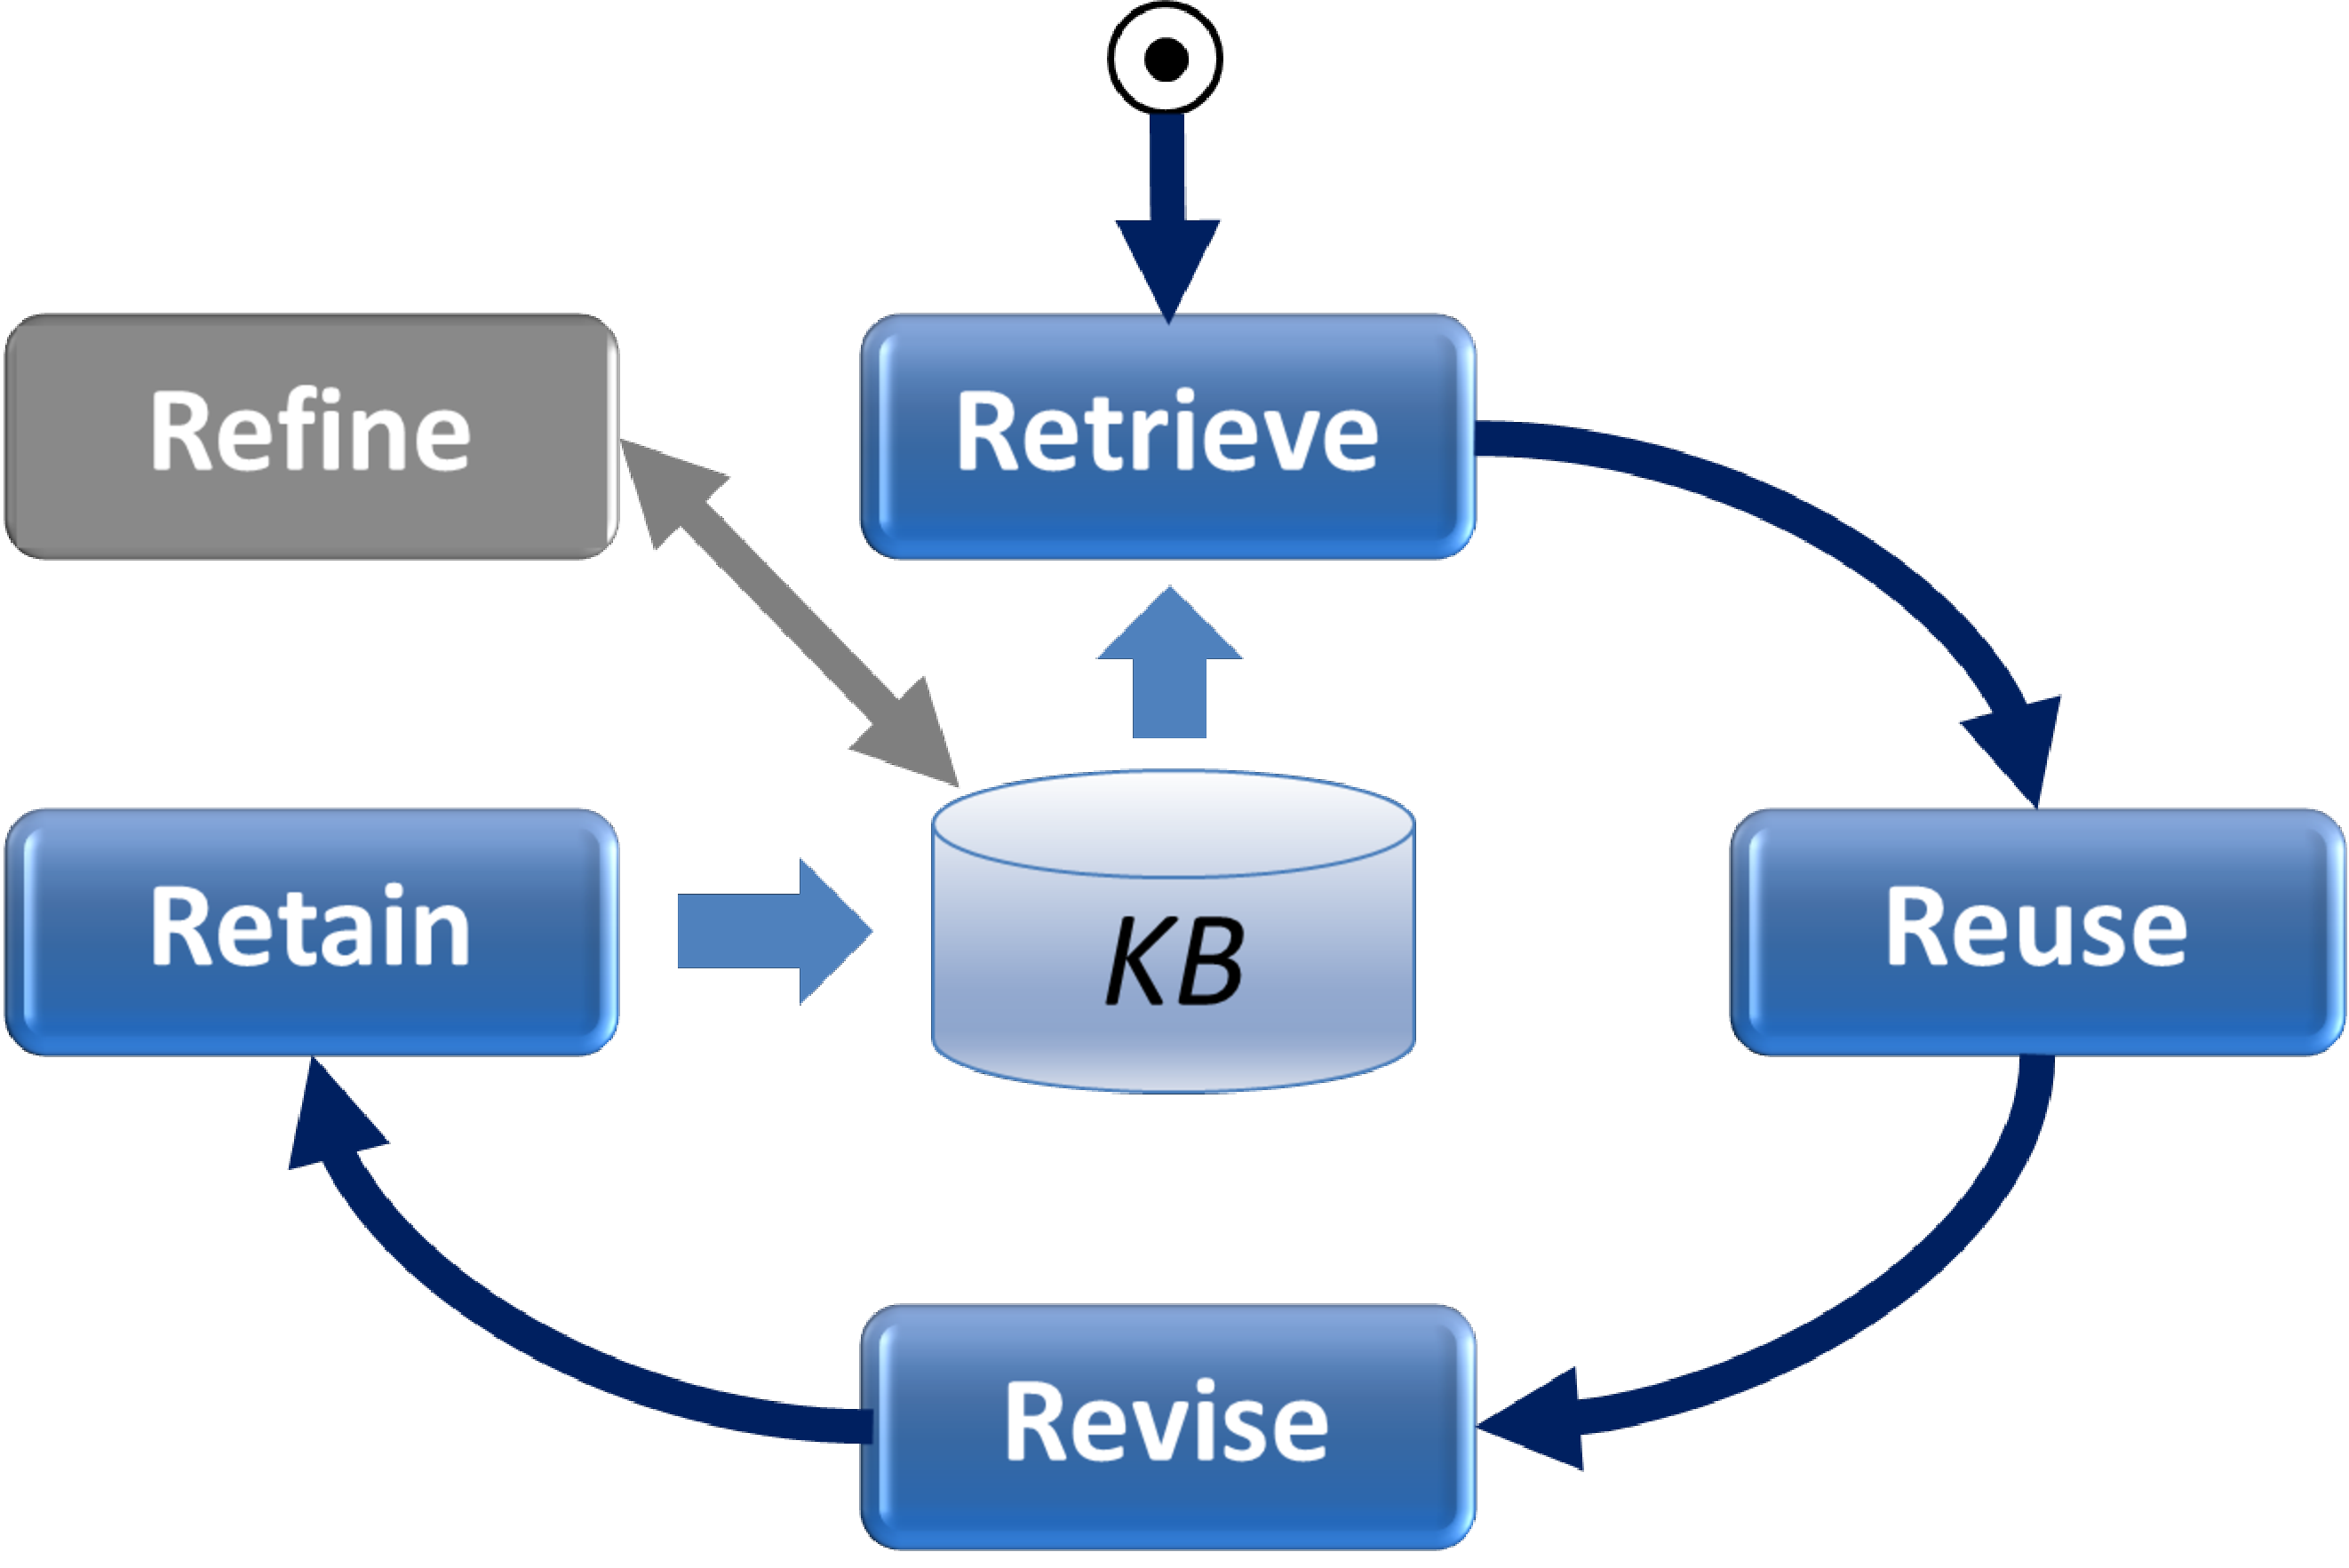
\includegraphics[scale=0.18]{CBR.pdf}
\caption{Main CBR steps and data-flow among them.}
\label{flow}
\end{figure}

In our proposed CBR logical architecture, the {\em Refine} process consists of a periodic check of the whole KB in order both to check the case base and to reconsider the knowledge used in the light of the results obtained, through properly defined quality metrics \cite{Reinartz2000}. 
Many different proposals exist in the literature on the definition of  the 
{\em Refine}. For instance, \cite{Tirri1996} suggests using Bayesian inference to determine  in a self-learning way the best mapping between cases and solutions. 
At the very essence of all approaches is always the usage of  the goodness evaluation function $g(\cdot)$  to assess, from a statistical point of view, the adequacy of the mapping between cases and solutions performed by the similarity function $sim(\cdot)$. 
For instance, it would be advantageous to determine, from the $KB$ content, which are the cases that were successfully solved by the application of a given strategy. This information should be used  to define updates to the similarity function. Similarly, the set of solutions techniques that worked well on similar cases should be explored. The analysis of these data may indicate the opportunity of deleting some tuples from the $KB$, to avoid repeating erroneous choices already done in the past.   
As pointed-out in \cite{Smyth1995}, to forget is an essential part of the learning in a CBR setting.  

\section{Problem definition} 
\label{prob}
We consider the problem of assigning tasks to a the available equipment of a manufacturing line. In our first approximation of the optimization problem, we will be considering a single machine that is available to process a flow of requests. 
In spite of an apparent simplicity, this scenario defines a complex optimization problem, which we shall detail in the following. 

We assume the load of the machine is to be scheduled over a fixed period of time, whose duration is $D$ days. The machine has a fixed processing capacity per day, which is denoted by $T$. Therefore, the total capacity for the whole scheduling period is $TD$. 
Requests for processing are known for the period, and we want to decide the order of execution of the requests on the machine. 
Let us denote with $r_1,r_2,\ldots,r_N$ the set of requests for the period. 
Request $r_i$, $i=1,2,\ldots,N$ is characterized by the following  parameters:
\begin{itemize}
\item The amount of processing time it requires to be completed, denoted by $t_i$, which can take any positive real value.
\item The due date by which the request processing must be completed, denoted by $d_i$, an integer in the set $\{1,2,\ldots,D\}$.
\item The value gained with the completion of the request within the due date, denoted by $v_i$, a real positive value;
\item a boolean property that says whether the execution of the request can be fractioned over time, denoted by $f_i$, which takes value $0$ for non-fractionable requests and value $1$ for fractionable ones. 
\end{itemize}
We assume that no gain is obtained for requests that are only partially processed. 

The problem of deciding which requests to process and optimize the total gain can be  formulated as an integer optimization problem.
Let us define the following variables: 
\begin{itemize}
\item 
$I_{ij}$, whose value is the time, within day j, at which the execution of of request $i$ starts execution, $i=1,2,\ldots,N$, $j=1,2,\ldots,D$. The variable takes values in the set $\{-1\} \cup [0,24)$, where the value $-1$ is used to indicate that the request $i$ does not have a processing time during day $j$. 
\item
$T_{ij}$,  whose value is the amount of time, within day $j$, that request $i$ is assigned the machine, $i=1,2,\ldots,N$, $j=1,2,\ldots,D$. The variable takes values in the in the interval $[0,24]$, where the value $0$ is used to indicate that the request $i$ does not have a processing time during day $j$. 
\item 
$X_i$, a binary decision variable which takes value $1$ if request $i$ is included in the scheduling and $0$ otherwise, $i=1,2,\ldots,N$. 
\end{itemize}


Then, the optimization problem  of maximizing the total gain for the period can be stated as the problem of finding the assignment to the  variables that maximizes the following objective function:
\begin{equation}
\sum_{i=1}^{N} X_i v_i
\end{equation}
subject to the following constraints:
\[
\left\{ 
\begin{array}{lcc}
\sum_{i=1}^N T_{i,j} \leq T, & \forall  j& (c1)  \\
\\
\sum_{j=1}^D T_{i,j} = X_i t_i, & \forall i& (c2)  \\
\\
 J^{max}_i   \leq  d_i,  & \forall i & (c3) \\
 \\
 24*(J^{max}_i-J^{min}_i)+I_{i,J^{max}_i}+ & \\
 + T_{i,J^{max}_i} -I_{i,J^{min}_i} = X_i t_i, &  \forall i \mbox{ $|$ } f_i=0  & (c4) \\
 \end{array}
 \right.
 \]
where $J^{max}_i$ and $J^{max}_i$ are functions  on the set 
$S_i=\{j | I_{i,j} \geq 0\}$, 
defined as follows: $J^{max}_i$ is the maximum index in $S_i$ if the set is not empty and $1$ otherwise, and $J^{min}_i$ is the minimum index in $S_i$ if the set is not empty and $1$ otherwise. 
The constraints $(c1)$ restrict the assignment to the variables in way that the daily workload does not exceed the capacity $D$ of the machine, the constraints $(c2)$ specify that each request selected for execution must be completed, $(c3)$ enforces the completion of the requests selected for execution by the deadline, and finally $(c4)$ imposes the sequential execution, with no interruptions, of all the non-fractionable requests selected for execution. 

It is important to notice that there may be cases of requests that cannot be  scheduled to meet their deadline under any possible assignment of processing time to the machine. This is the case when the processing time $t_i$ of request $r_i$ is such that 
\begin{equation}
\label{unfeasible}
t_i > d_i T
\end{equation} 
Obviously, all requests satisfying the condition above have to be removed from the workload before initiating any attempt to solve the optimization problem. 

To make an example of an instance of the problem, suppose we have a planning horizon of 5 days, i.e. D = 5, the daily processing capacity of the machine being T = 1 (day). Let us suppose the workload to be scheduled for the week consists of the items listed  in   Table \ref{example}. 
\begin{table}[h!]
\centering
\begin{tabular}{|cccrc|}
\hline
{\bf Request} & {\bf Processing} & {\bf Deadline} & {\bf Value} & {\bf Fractionable} \\ \hline
$r_1$ & 0.25 & 3 & 100 & 0 \\ \hline
$r_2$ & 2.25 & 5 & 300 & 1 \\ \hline
$r_3$ & 0.10 & 2 & 150 & 0 \\ \hline
$r_4$ & 2.50 & 2 & 100 & 1 \\ \hline
$r_5$ & 0.50 & 1 & 50 & 0 \\ \hline
$r_6$ & 1.50 & 5 & 50 & 1 \\ \hline
\end{tabular}
\caption{Example of workload submitted for scheduling.}
\label{example}
\end{table}
Notice that request $r_4$ cannot be processed while meeting the deadline, because  its parameters satisfy eq.\ref{unfeasible}. 
Therefore, no assignment to the machine is tried for $r_4$. The processing of the remaining 5 requests can be scheduled according to the solution proposed in Figure \ref{solution}. 
\begin{figure}[h!]
\centering
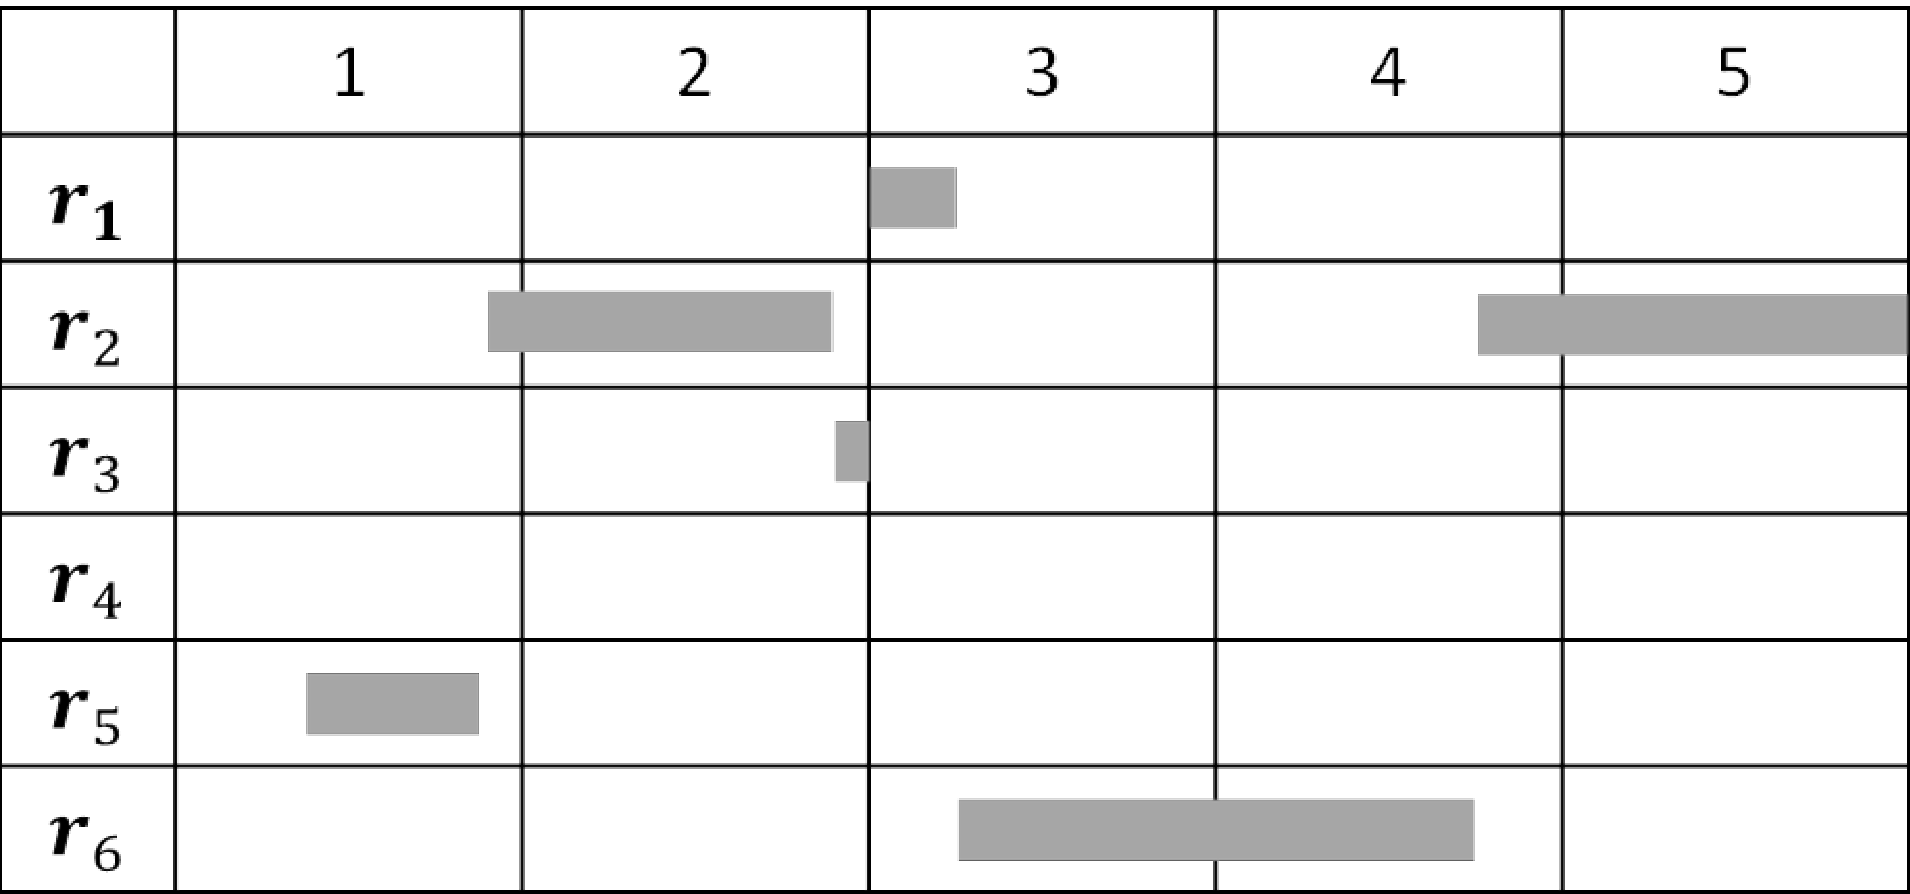
\includegraphics[scale=0.2]{Schedule.pdf}
\caption{A possible optimal scheduling solution for the case in Table \ref{example}.}
\label{solution}
\end{figure}
All requests would be processed in an non-preemptable fashion, apart for $r_2$, whose execution is split across two non-consecutive days.  The total gain of this assignment is 650, which is the maximum possible gain for the workload specified in Table \ref{example}.  
 

\section{Algorithmic approaches to the solution}
\label{alg}

The optimization problem stated in the previous section is a complex one, due to the need  of determining integer assignments to some of the variables, and to the form of the constraints $(c4)$. In its essence, it is a kind of multi-knapsack problem, with a constraint on the daily capacity. However, the existence of factors that may provide 
for an increased flexibility in the schedule of the some requests, i.e. their fractionability, may lead to heuristic solution schemes that could provide good, not necessarily  optimal solutions at a reduced computational time. 

The objective of this section is to present a set of solution algorithms that provide exact or approximate solutions to the decision problem. These algorithms will provide the input resources for the meta-solution scheme applied inside the CBR. 
 
\subsection{Optimal solution algorithm}

Pseudo-code for a dynamical programming solution algorithm. 
\small
\lstset{tabsize=2}

\begin{lstlisting}[mathescape]

knapsack(v,w,n,W){
for i=1 to n
	c[i,0]=0
	for j=1 to W
		if w[i-1] <= j
			c[i,j] = max(c[i-1,j], 
			         c[i-1,j-w[i-1]]+v[i-1])
		else
			c[i,j]=c[i-1,j]
		endif
	endfor
endfor
}
\end{lstlisting}
\normalsize

\subsection{Heuristic solution algorithms}
In this section we present the rationale of a family of heuristic solution algorithms, which attempt to maximize the value of the assignment by exploiting the fractionability of the requests. We begin by considering the simplest case when all requests are fractionable, i.e. $f_i=1, \forall i$. 

\subsubsection{All fractionable requests} 
In this scenario, we consider two distinct heuristics to solve the decision problem, depending on whether the workload is feasible, i.e. all requests can be satisfied, or unfeasible, i.e. it is only possible to execute a subset of the requests. 

Let us denote by $E_j$ the set of requests that have a deadline $d_j$ less or equal than day $j$, $j=1,2,\ldots,D$. 
If the following conditions are satisfied by the workload, 
\begin{equation}
j T  \geq \sum_{j \in E_i}t_j , \forall j=1,2,…,D
\label{capacity}
\end{equation} 
 then, the instance of the problem allows satisfying all requests. 
 An algorithm to find a feasible  assignment for all the requests  works according to an Earliest Deadline First criterion, as follows: 
 \small
 \begin{lstlisting}[mathescape]
EarliestFirst(workload){
p_times =($t_1,t_2,\ldots,t_N$)
deadlines=($d_1,d_2,\ldots,d_N$)
for j=1 to D
	used_capacity=0
	while (used_capacity<T) 
		 i = min(deadlines) 
		 new_p_time=min$\{t_i,T\}$
		 p_times[i]=p_times[i]-new_p_time
		 if p_times[i]=0 
		 	deadlines[i]=$\infty$
		endif
		$I_{ij}$=used_capacity
		$T_{ij}$=new_p_time
		used_capacity=used_capacity+new_p_time
	endwhile
endfor
}
\end{lstlisting}
\normalsize

 This algorithm returns a feasible assignment for all the requests, by partitioning the execution of tasks so that the completion times are ordered according to the deadlines.
 It is easy to show that all the requests are scheduled in a way that they are all processed before the respective deadline. If not so, because the algorithms sequentially {\em fills-in} the capacity of the days, it would mean that the the incremental capacities along the period are not sufficient to schedule the requests, that is, it would contradict the conditions stated by (\ref{capacity}).
 
When the conditions at (\ref{capacity}) are not satisfied, still in the case of all fractionable request, the optimization problem starts to show its complexity. Indeed, it is not said that all requests are processable before their deadline, and the maximum total gain can be less than the sum of the $v_i$, $i=1,2,\ldots.n$. 
When $TD <  \sum_{i=1} ^N t_j$  holds, it is certain that not all the workload is feasible. 
However, even in this case, because of the fractionable nature of the requests, we can easily determine a an heuristic to assign the machine, based on a highest density value criterion.  
\small
\begin{lstlisting}[mathescape]
HighestValueDensityFirst{
densities=($g_1/t_1, g_2/t_2, \ldots,g_N/t_N$)
new_wkld=$\emptyset$
total_proc=0
while (total_proc $\leq$ TD) 
	i = $\{j { }|{ }  $densities$[j]$ $\geq$ densities$[h]$, 
	    $h=1,2,\ldots,N\}$ 
	new_wkld=new_wkld$\cup \{i\}$
	total_proc=total_proc+$t_i$
	densities[i]=0
endwhile
EarliestFirst(new_wkld)
} 
\end{lstlisting}
\normalsize

\subsubsection{Mixed fractionable and non-fractionable requests} 
  

  
 



\section{CBR application to the problem}
\label{inst}
In this section we describe how the various CBR steps defined in Section \ref{cbr} are to be instantiated with the aim  of solving our manufacturing optimization problem {\em to be done....} 

\subsection{Retrieve process} 

In the specific context of the scheduling problem, the Retrieve process of CBR finds the $N>0$ cases saved in the KB which are the most similar to the case being processed. 
To this goal, it requires the definition of a {\em similarity} function. 
We assume that the case has been checked for the existence of non-feasible requests, as defined in (\ref{unfeasible}), and proceed to  define the similarity between cases as being based on the following parameters: 
\begin{itemize}
\item  the percentage of fractionable cases that exist in the case, which we denote by $pf$; 
\item the estimated utilization that the case would determine on the machine of the machine, computed as $min(\sum_{i=1}^N t_i / TD,100\%)$, which we denote by $ut$
\item the percentage of days that the workload satisfies conditions (\ref{capacity}), which we denote by $cp$. 
\end{itemize}
Each of the parameters listed above is a number in the interval $[0,1]$. 

Let us denote by $pf_{new}, ut_{new}$ and $cp_{new}$ the values of the three parameters for the case under processing by the CBR. 
Then, a similarity between  the case at hand and any case $i$ stored in the $KB$ could be determined by the evaluation of the following function: 
\[
sim(new,i)=\frac{1}{3}\left( w_{pf}(1-|pf_{new}-pf_i|)+\right.
\]
\begin{equation}
\left.+ w_{ut}|ut_{new}-ut_i|
+w_{cp}|cp_{new}-cp_i| \right)
\end{equation}

A threshold lower-bound value $\sigma$ is defined, which allows recognizing as similar only those cases such that $sim(new,i)\geq \sigma$.

\subsection{Reuse process}
The Reuse receives the similar cases found by the Retrieve an determines which solution strategy is to be applied for the case to be solved. 

In the event that no similar cases are found in the $KB$, the Reuse simply chooses the default strategy $S_0$. Otherwise, it finds the returned case $i$ that obtained the best score in the $g(\cdot)$ function, and selects for reuse the strategy $S_j$ that had been applied  to the solution of $i$. 
The goodness evaluation function $g(\cdot)$ is implemented as an approximation of the distance between the scheduling solution find by the CBR for the case and its optimal solution. We shall be back later on to the exact definition of the goodness function. 

The Reuse calls the solution strategy  $S_j$, which returns the proposed scheduling for the case at hand. 

\subsection{Revise process}
The Revise checks the quality of the solution returned by the Reuse, and determines if it is of an acceptable quality. To do so, it evaluates the $g(\cdot)$
function and compares it with the average value of the same function, computed over the set of the $N$ cases found in the Retrieve step. If the score for the new case is at least as good as the average, the proposed solution passes the check, otherwise it is rejected, and the default strategy $S_0$ is invoked to find an alternative solution to the problem. 

\subsection{Retain process}
The Retain is responsible for updating the $KB$ with the new piece of information the CBR system learned while approaching the solution of the new case. 
A tuple is constructed, formed by
\begin{itemize}
\item the parameters that specify the new case;
\item the strategy that was applied for its execution;
\item the result of the evaluation of the goodness function for the case.
\end{itemize} 
This tuple is added to the $KB$, and the CBR cycle is completed.

\subsection{Refine process}

\subsection{The goodness function}
{\em Es posible usar dos distinctas funciones, een entrenamiento y en operaci�n: la primera podr�a hacer referencia al valor optimo, la segunda ..}
 




\subsection{Refine process}
\section{Preliminary result evaluation}
\label{outc}

\section{Conclusions and future work}
\label{concl}

\bibliography{CBR}

\end{document}





